\documentclass[xcolor=dvipsnames]{beamer}
\usetheme{Madrid}


\setbeamertemplate{navigation symbols}{}
%\setbeamertemplate{headline}{}

%\setbeamertemplate{frametitle}{\insertpagenumber}
\setbeamertemplate{footline}[frame number]
%\setbeamersize{text margin left=7mm}
%\setbeamersize{text margin right=7mm}

\usepackage{hyperref}
%\hypersetup{colorlinks, linkcolor=black}

\usepackage{times}

\usepackage{xltxtra}
\setsansfont{Calibri}
\setmonofont{Consolas}

\usepackage{minted}


\author{Jan Dědek}

\institute[MFF UK] % (optional, but mostly needed)
{
  Department of Software Engineering\\
	Faculty of Mathematics and Physics\\
	Charles University in Prague
}

\date[DEDEK-PHD, 2012]
{
Defence of Doctoral Thesis\\21\textsuperscript{st} September\\2012
}

\title{Semantic Annotations}

\begin{document}

\begin{frame}
  \titlepage
\end{frame}

\definecolor{DarkGreen}{rgb}{0,.392,0}
\definecolor{DarkMagenta}{rgb}{.545,0,.545}
\definecolor{DarkCyan}{rgb}{0,.545,.545}


\def \colorManual    {Brown}
\def \colorLearning  {DarkGreen}
\def \colorShareable {DarkCyan}
\def \colorFuzzy     {DarkMagenta}
\def \mysetbeamercolor [#1]#2 {\setbeamercolor{#1}{fg=#2}}

\mysetbeamercolor[colorManual]{\colorManual}
\mysetbeamercolor[colorLearning]{\colorLearning}
\mysetbeamercolor[colorShareable]{\colorShareable}
\mysetbeamercolor[colorFuzzy]{\colorFuzzy}


\def \themecolor #1 {\setbeamercolor*{titlelike}{parent=palette primary, bg=#1}}
\def \themetext [#1]#2 {{\usebeamercolor{#1}{\color{fg}\textbf{#2}}}}
\def \resetcolor {\setbeamercolor*{titlelike}{parent=palette primary}}



\definecolor{mybkg}{RGB}{240,240,240}
\setbeamercolor{block title}{bg=OliveGreen}
\setbeamercolor{block body}{bg=mybkg}

\begin{frame}{Outline}
  \tableofcontents
\end{frame}

\section{Introduction} 
\subsection{Information Extraction} 
\frame{\tableofcontents[currentsubsection]}
\begin{frame}{Information Extraction (Problem)}  
\begin{itemize}
	\item Let's have a text describing an acquisition event.
	\medskip
	\framebox{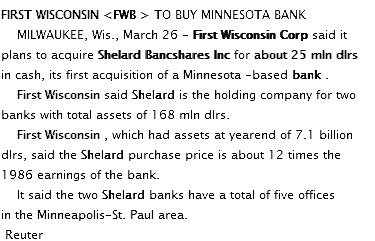
\includegraphics[width=0.6\hsize]{img/acquisitions_plain.png}}
	\item What was the object of the acquisition?
	\item Who was the buyer?
	\item What was the deal amount?
\end{itemize}
\end{frame}

\begin{frame}{Information Extraction (Solution)}  
\begin{itemize}
	\item Information Extraction tools can identify and extract such information.
	%\begin{itemize}
		%\item Of course not 100\% accurete...
	%\end{itemize}
	\medskip
	\framebox{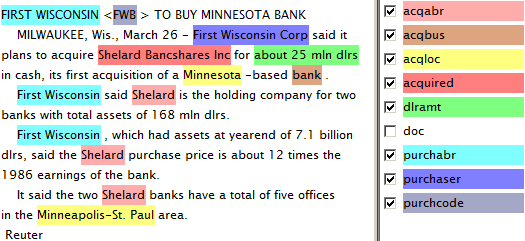
\includegraphics[width=0.85\hsize]{img/acquisitions_annotated.png}}
	%\item The tools can also interpret such information in terms of a \alert{Semantic Web Ontology}.
\end{itemize}
\end{frame}

\begin{frame}{Information Extraction (Czech Example)}  
\begin{itemize}
	\item Information Extraction tools can identify and extract such information.
	%\begin{itemize}
		%\item Of course not 100\% accurete...
	%\end{itemize}
	\medskip
	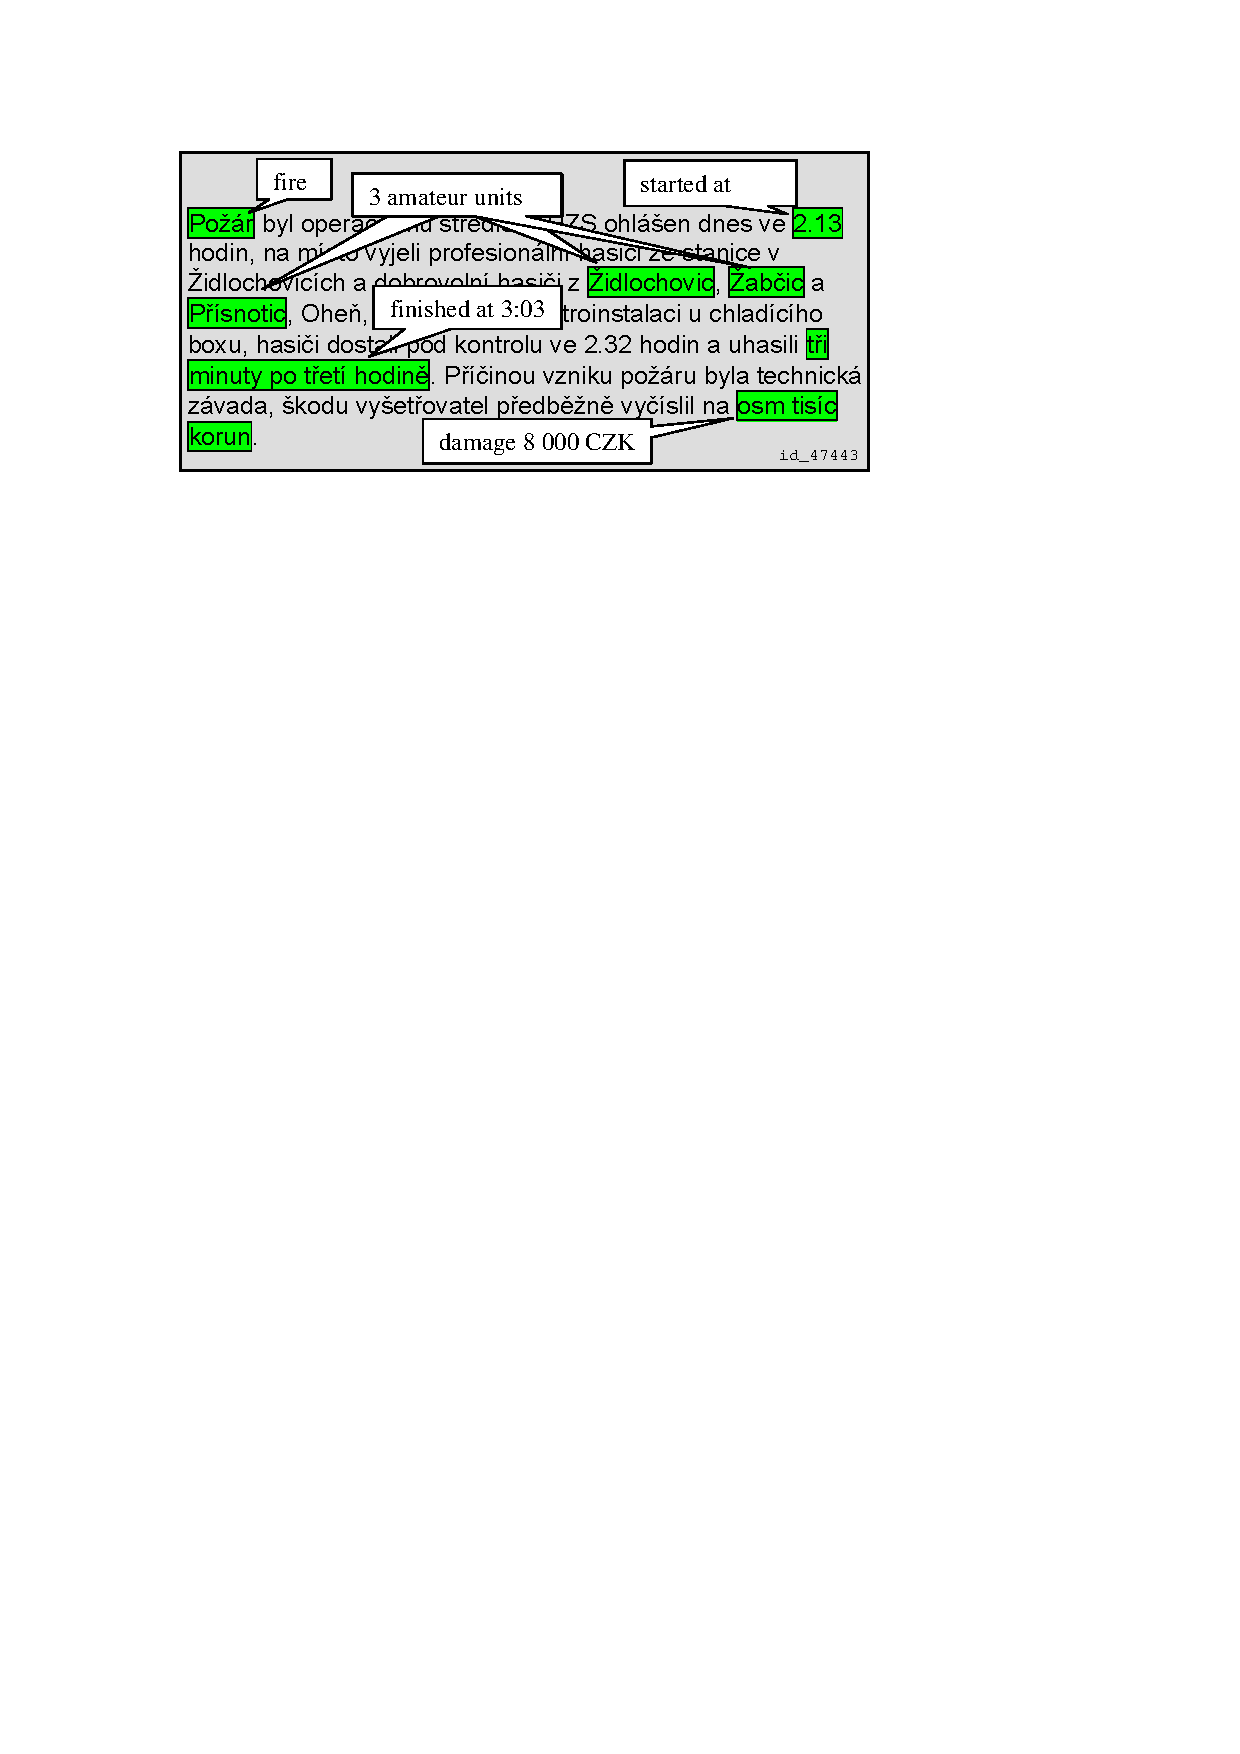
\includegraphics[width=0.85\hsize]{img/fireman_annotated}
	%\item The tools can also interpret such information in terms of a \alert{Semantic Web Ontology}.
\end{itemize}
\end{frame}

\subsection{Deep Language Parsing} 
\begin{frame}{Deep Language Parsing (Czech Example)}  
\begin{itemize}
	\item Linguistic tools perform automated linguistic analysis.
	\item Producing so called \emph{dependency trees}.
	%\begin{itemize}
		%\item Of course not 100\% accurete...
	%\end{itemize}
	\medskip
	\framebox{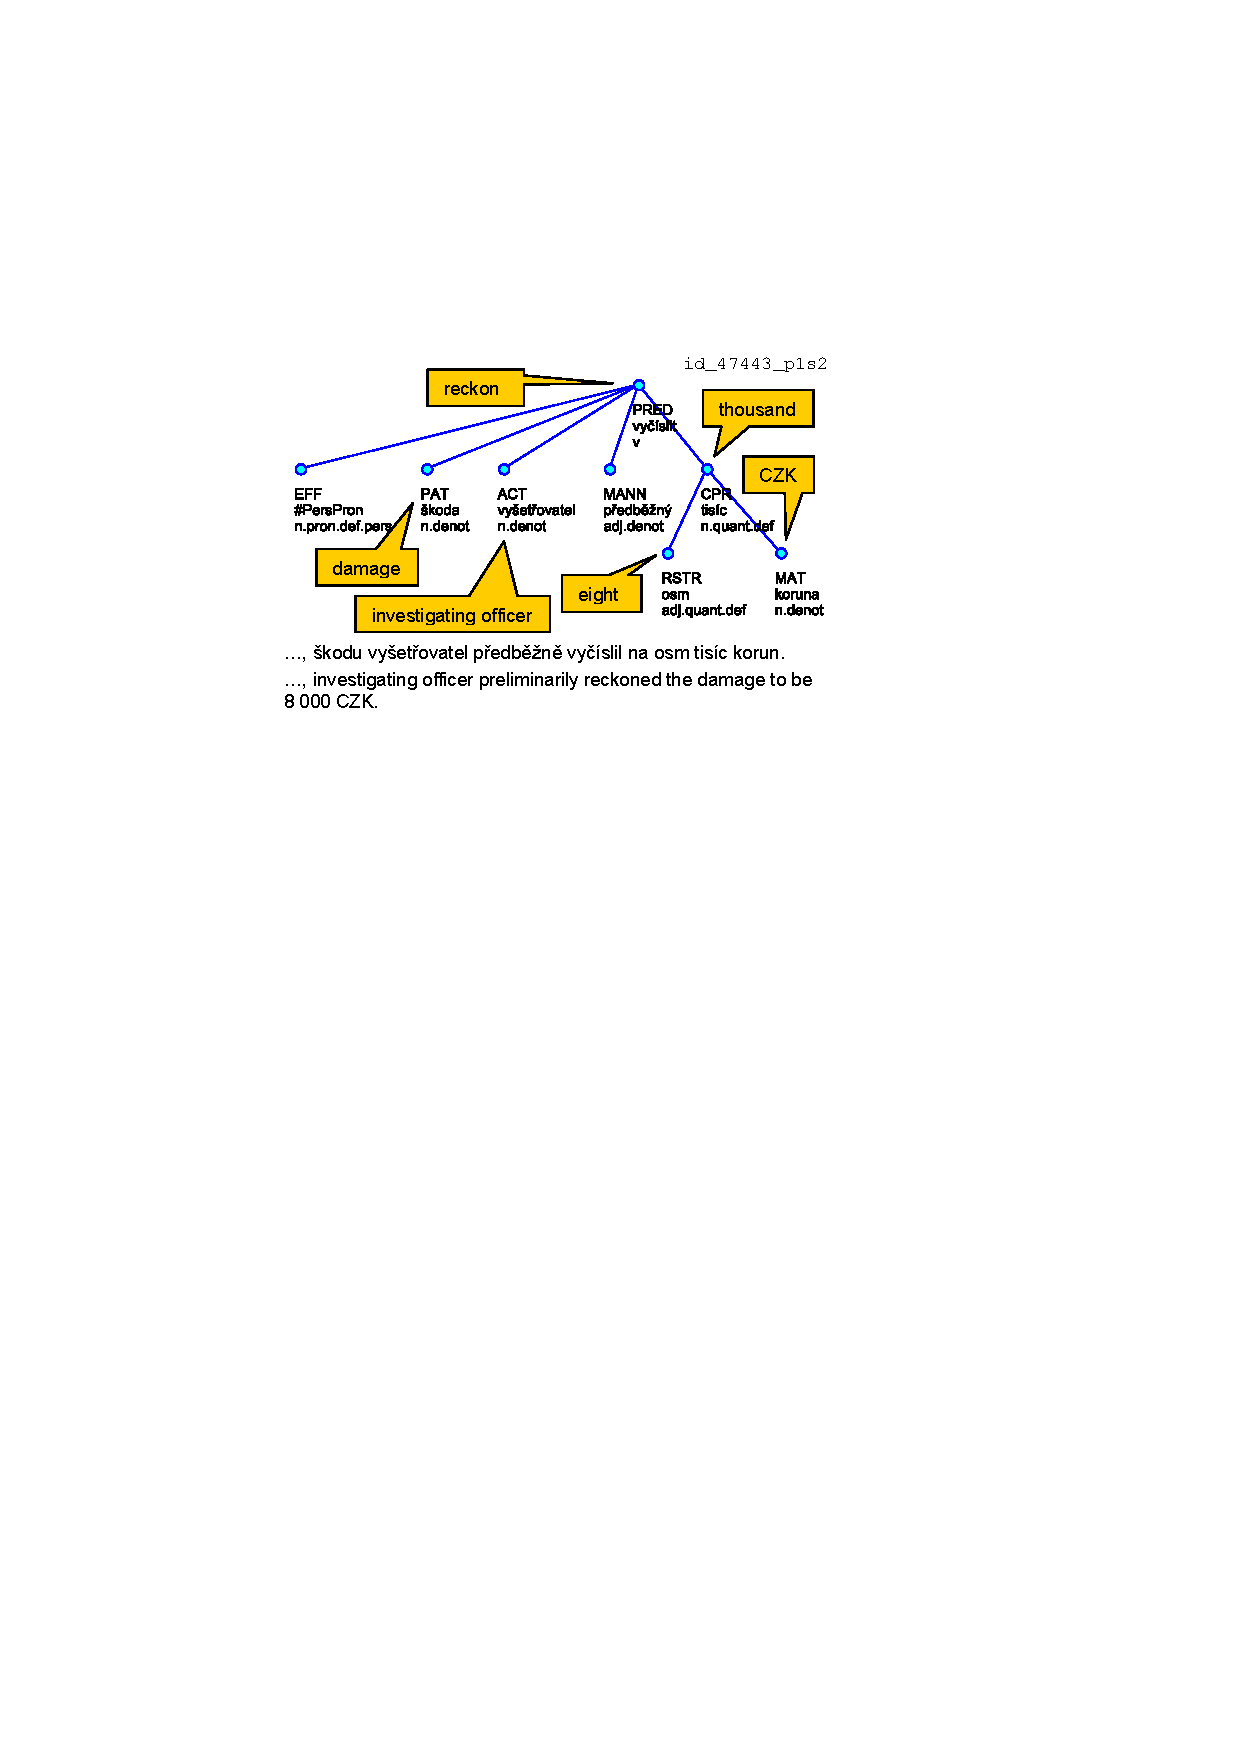
\includegraphics[width=0.85\hsize]{img/tree}}
	%\item The tools can also interpret such information in terms of a \alert{Semantic Web Ontology}.
\end{itemize}
\end{frame}

\begin{frame}{Layers of linguistic annotation in PDT}
\begin{columns}
\column{.5\textwidth}
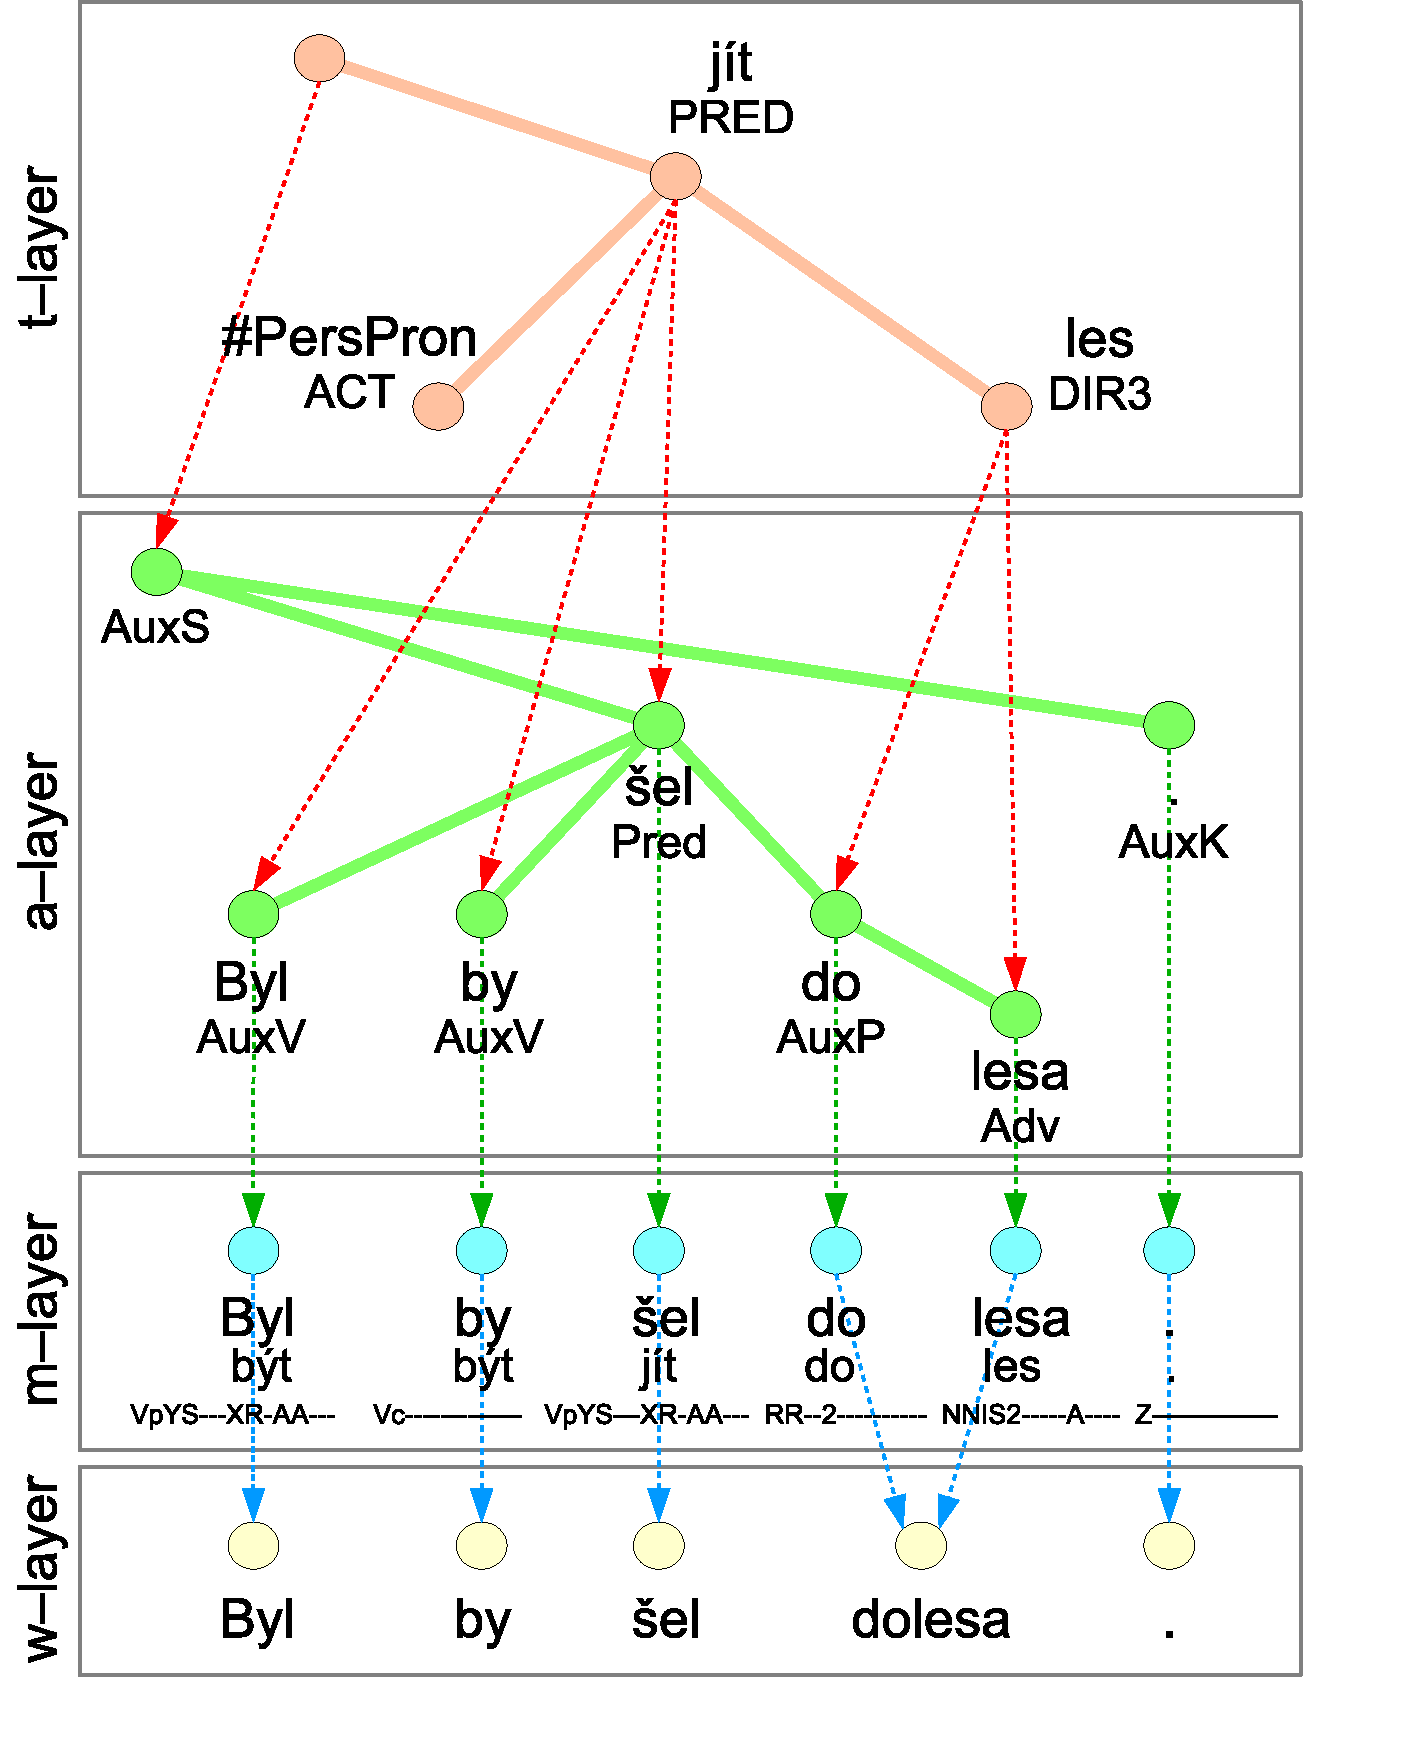
\includegraphics[height=0.9\vsize]{img/PDT_layers}
\column{.5\textwidth}
\begin{itemize}
	\item Tectogrammatical layer
	\item Analytical layer
	\item Morphological layer
\end{itemize}
\begin{itemize}
	\item PDT 2.0 on-line:\\\centerline{\scriptsize\url{http://ufal.mff.cuni.cz/pdt2.0/}} 
\end{itemize}
\vspace{2cm}
\emph{Sentence:}
\medskip
\\Byl by šel dolesa.
\\He-was would went toforest.
\end{columns}
\end{frame}


\subsection{Inductive Logic Programming} 

\begin{frame}{Inductive Logic Programming}
\begin{itemize}
	\item Learning examples $E=P\cup N$ (Positive and Negative)	
	\begin{itemize}
		\item E.g. relevant and irrelevant pieces of text w.r.t. particular extraction task
	\end{itemize}	
	\item Background knowledge $B$
	\begin{itemize}
		\item E.g. linguistic structure connecting individual words
	\end{itemize}	
	\item ILP task: To find logical program or hypothesis $H$ such that all positive examples are covered and none negative
$$
(\forall e\in P)(B\cup H\models e) \ \ \&\  \ (\forall n\in N)(B\cup H\not\models n).
$$
	\begin{itemize}
		\item E.g. to find common pattern (in the linguistic structure) present around every relevant piece of text and none irrelevant.
	\end{itemize}	
\end{itemize}
\end{frame}


\subsection{Organization of this Presentation} 
\frame{\tableofcontents[currentsubsection]}

\begin{frame}{Four Main Topics}

\begin{itemize}
	\item \themetext[colorManual]{Manual Design of Extraction Rules}
	\item \themetext[colorLearning]{Induction of Extraction Rules}
	\item \themetext[colorShareable]{Shareable Extraction Ontologies}
	\item \themetext[colorFuzzy]{Fuzzy ILP Document Classification}
\end{itemize}

\end{frame}


\themecolor{\colorManual}
\begin{frame}{Manual Design of Extraction Rules}
Slides about the topic \emph{Manual Design of Extraction Rules} will have \themetext[colorManual]{brown }  headline background.
\end{frame}

\themecolor{\colorLearning}
\begin{frame}{Induction of Extraction Rules}
Slides about the topic \emph{Induction of Extraction Rules} will have \themetext[colorLearning]{green }  headline background.
\end{frame}

\themecolor{\colorShareable}
\begin{frame}{Shareable Extraction Ontologies}
Slides about the topic \emph{Shareable Extraction Ontologies} will have \themetext[colorShareable]{cyan }  headline background.
\end{frame}

\themecolor{\colorFuzzy}
\begin{frame}{Fuzzy ILP Document Classification}
Slides about the topic \emph{Fuzzy ILP Document Classification} will have \themetext[colorFuzzy]{magenta }  headline background.
\end{frame}

\resetcolor
\begin{frame}{Ordinary}
\end{frame}


\section{Contents}
\subsection{Manual Design of Extraction Rules}
\themecolor{\colorManual}
\frame{\frametitle{Manual Design of Extraction Rules} \tableofcontents[currentsubsection]}


\begin{frame}[plain]
\begin{columns}
\column{.67\textwidth}
%\centerline{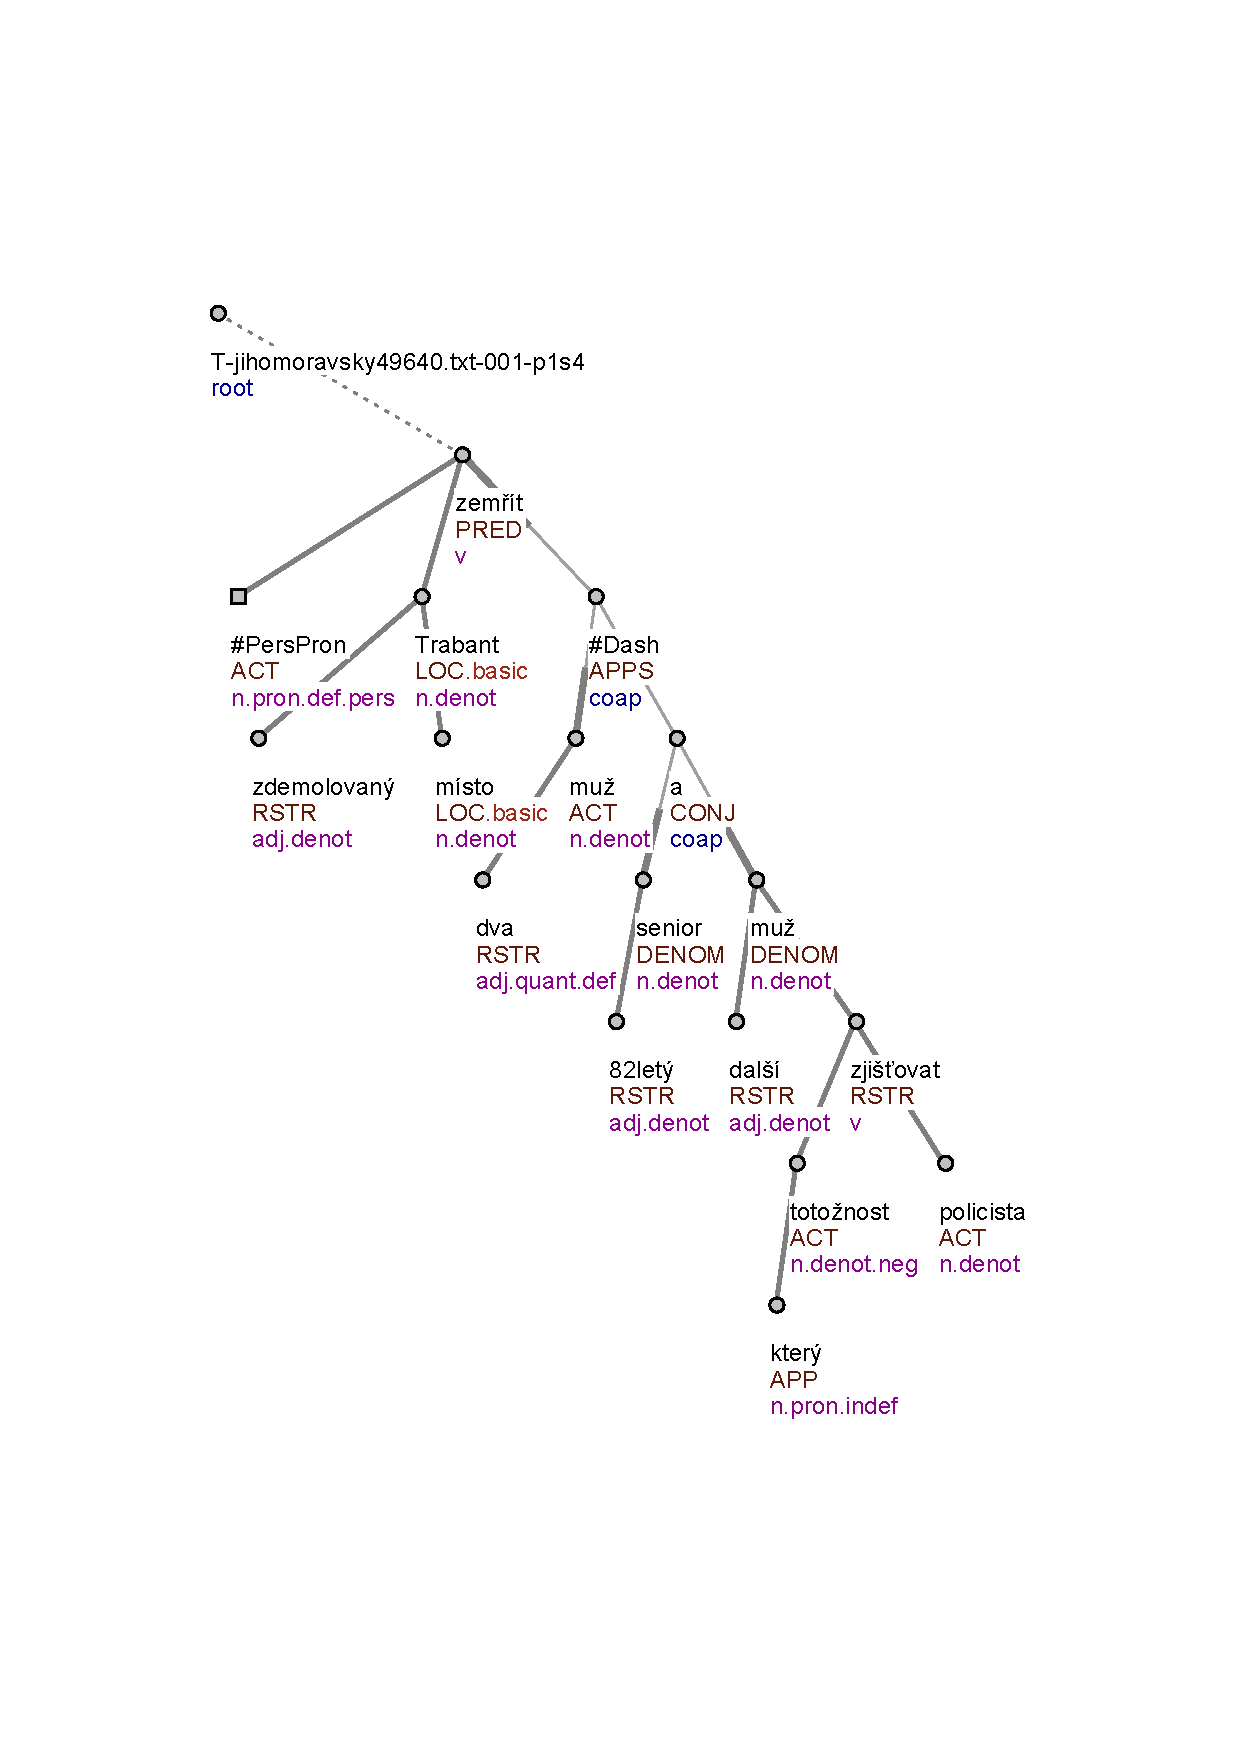
\includegraphics[height=1.1\vsize,width=\hsize]{img/TectogramaticalTree}}
\centerline{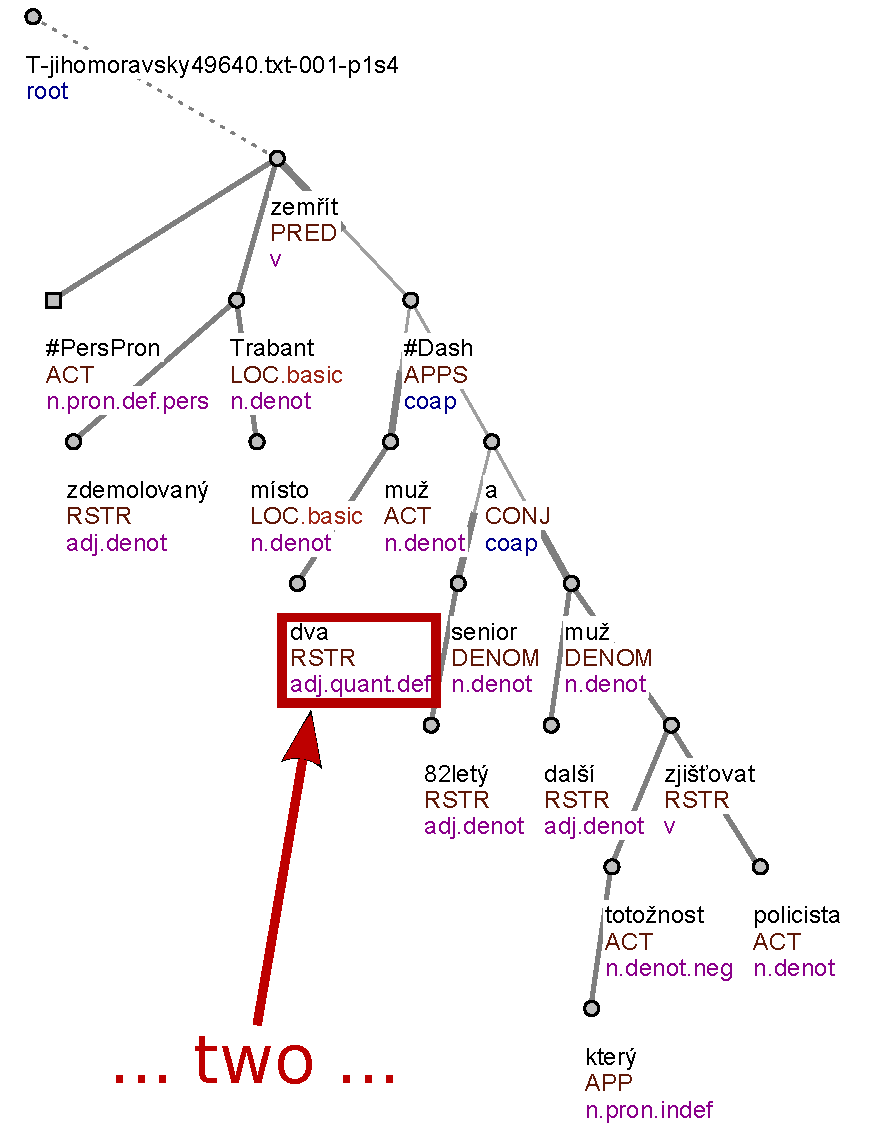
\includegraphics[height=1.1\vsize]{img/Two_Tree}}
\column{.33\textwidth}
\begin{itemize}
	\item How to extract the information about \alert{two dead} people?
\end{itemize}
\vspace{2cm}
\end{columns}
\end{frame}



\begin{frame}{Extraction rules -- Netgraph queries}
\begin{center}
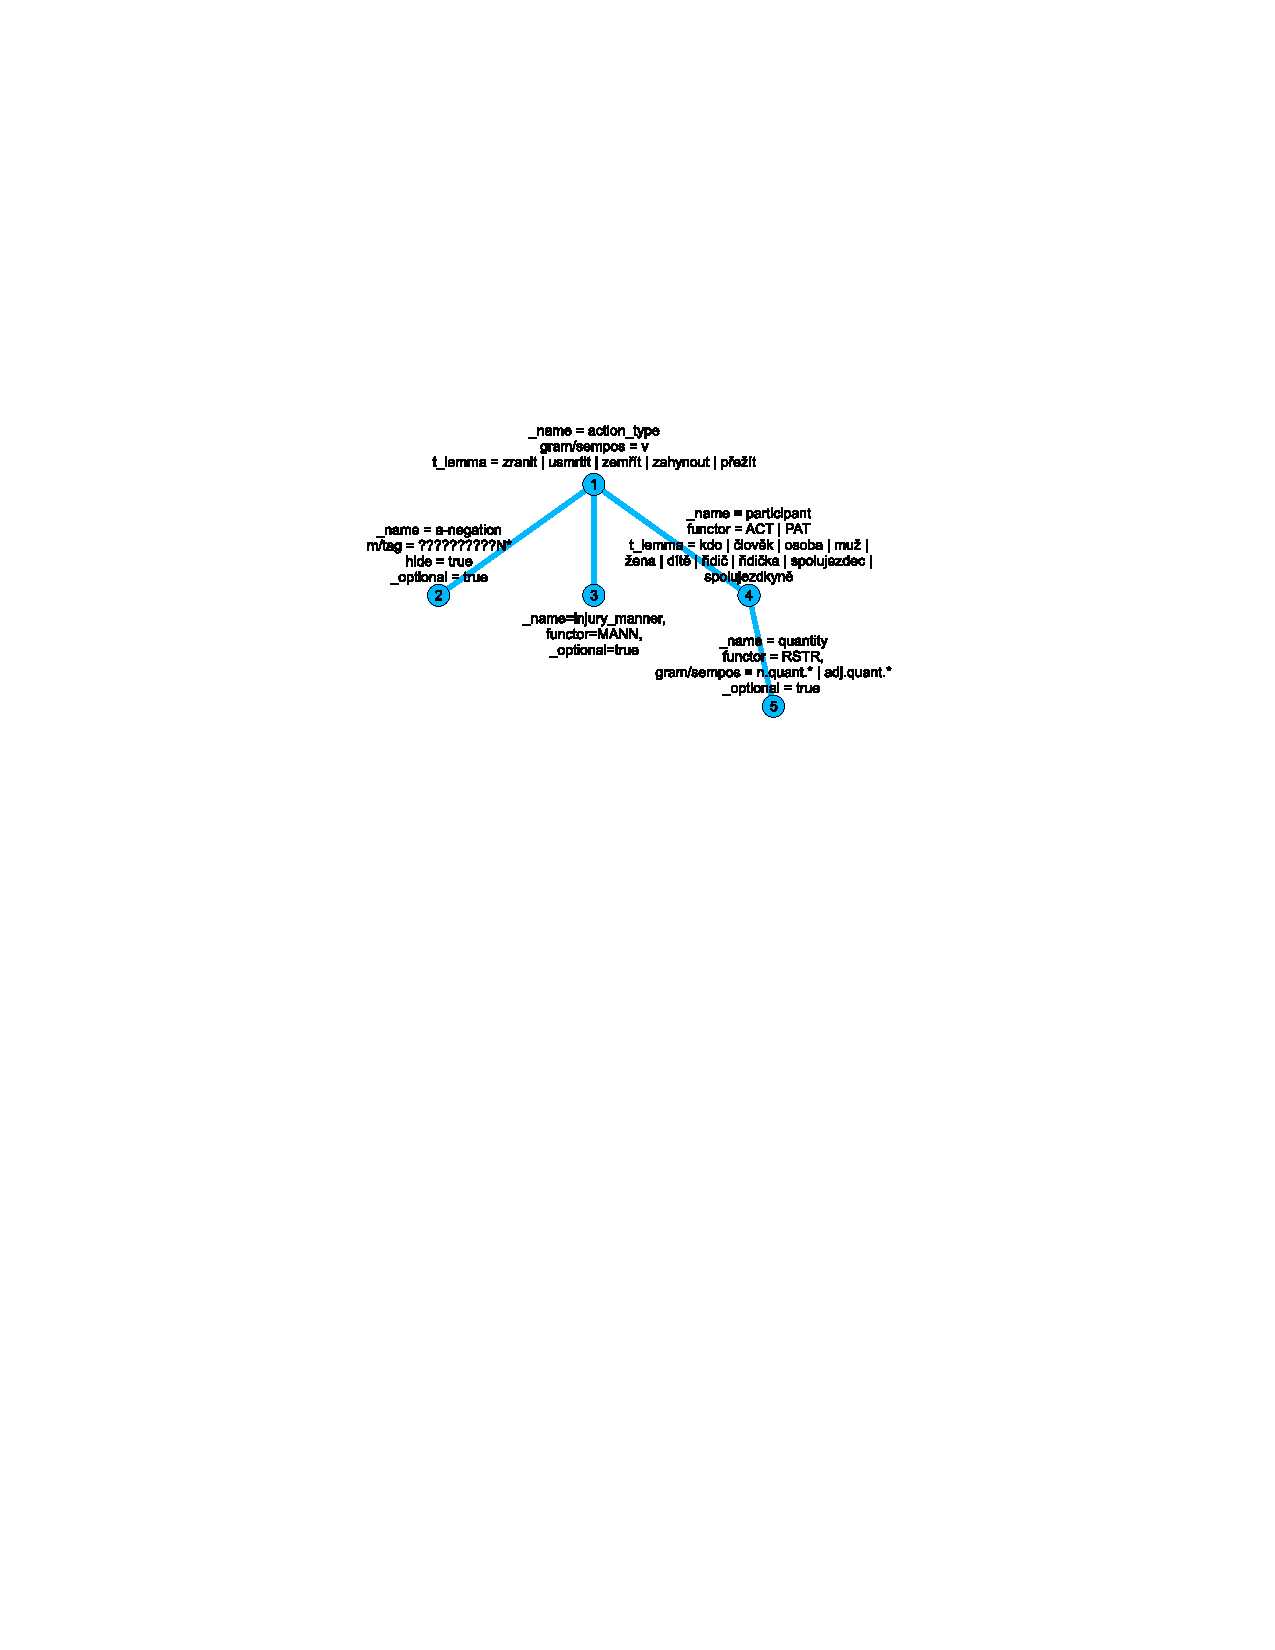
\includegraphics[height=0.6\vsize]{img/extract_patern}
\end{center}
\begin{itemize}
	\item Tree patterns on \alert{shape} and \alert{nodes} (on node attributes).
	\item Evaluation gives \alert{actual matches} of particular nodes.
	\item \alert{Names} of nodes allow use of references.
\end{itemize}
\end{frame}


\begin{frame}{Raw data extraction output}
%\begin{center}
\centerline{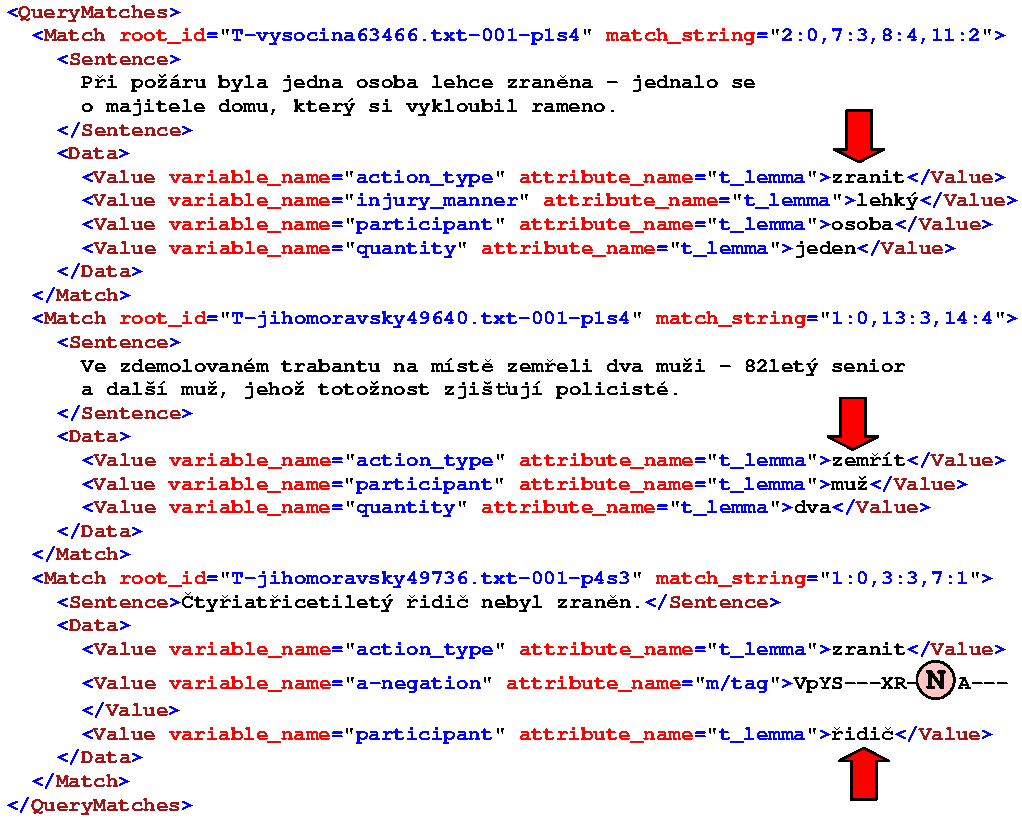
\includegraphics[height=0.18\vsize]{img/OutputQueryMatches}}
%\end{center}

{\scriptsize
\textbf{SELECT} \alert{action\_type}.t\_lemma, \alert{a-negation}.m\/tag, 
\alert{injury\_manner}.t\_lemma, \alert{participant}.t\_lemma,
\alert{quantity}.t\_lemma \textbf{FROM} \emph{***extraction rule***} 
}
\end{frame}

\begin{frame}{Extraction rules -- Environment Protection Use Case}
\begin{center}
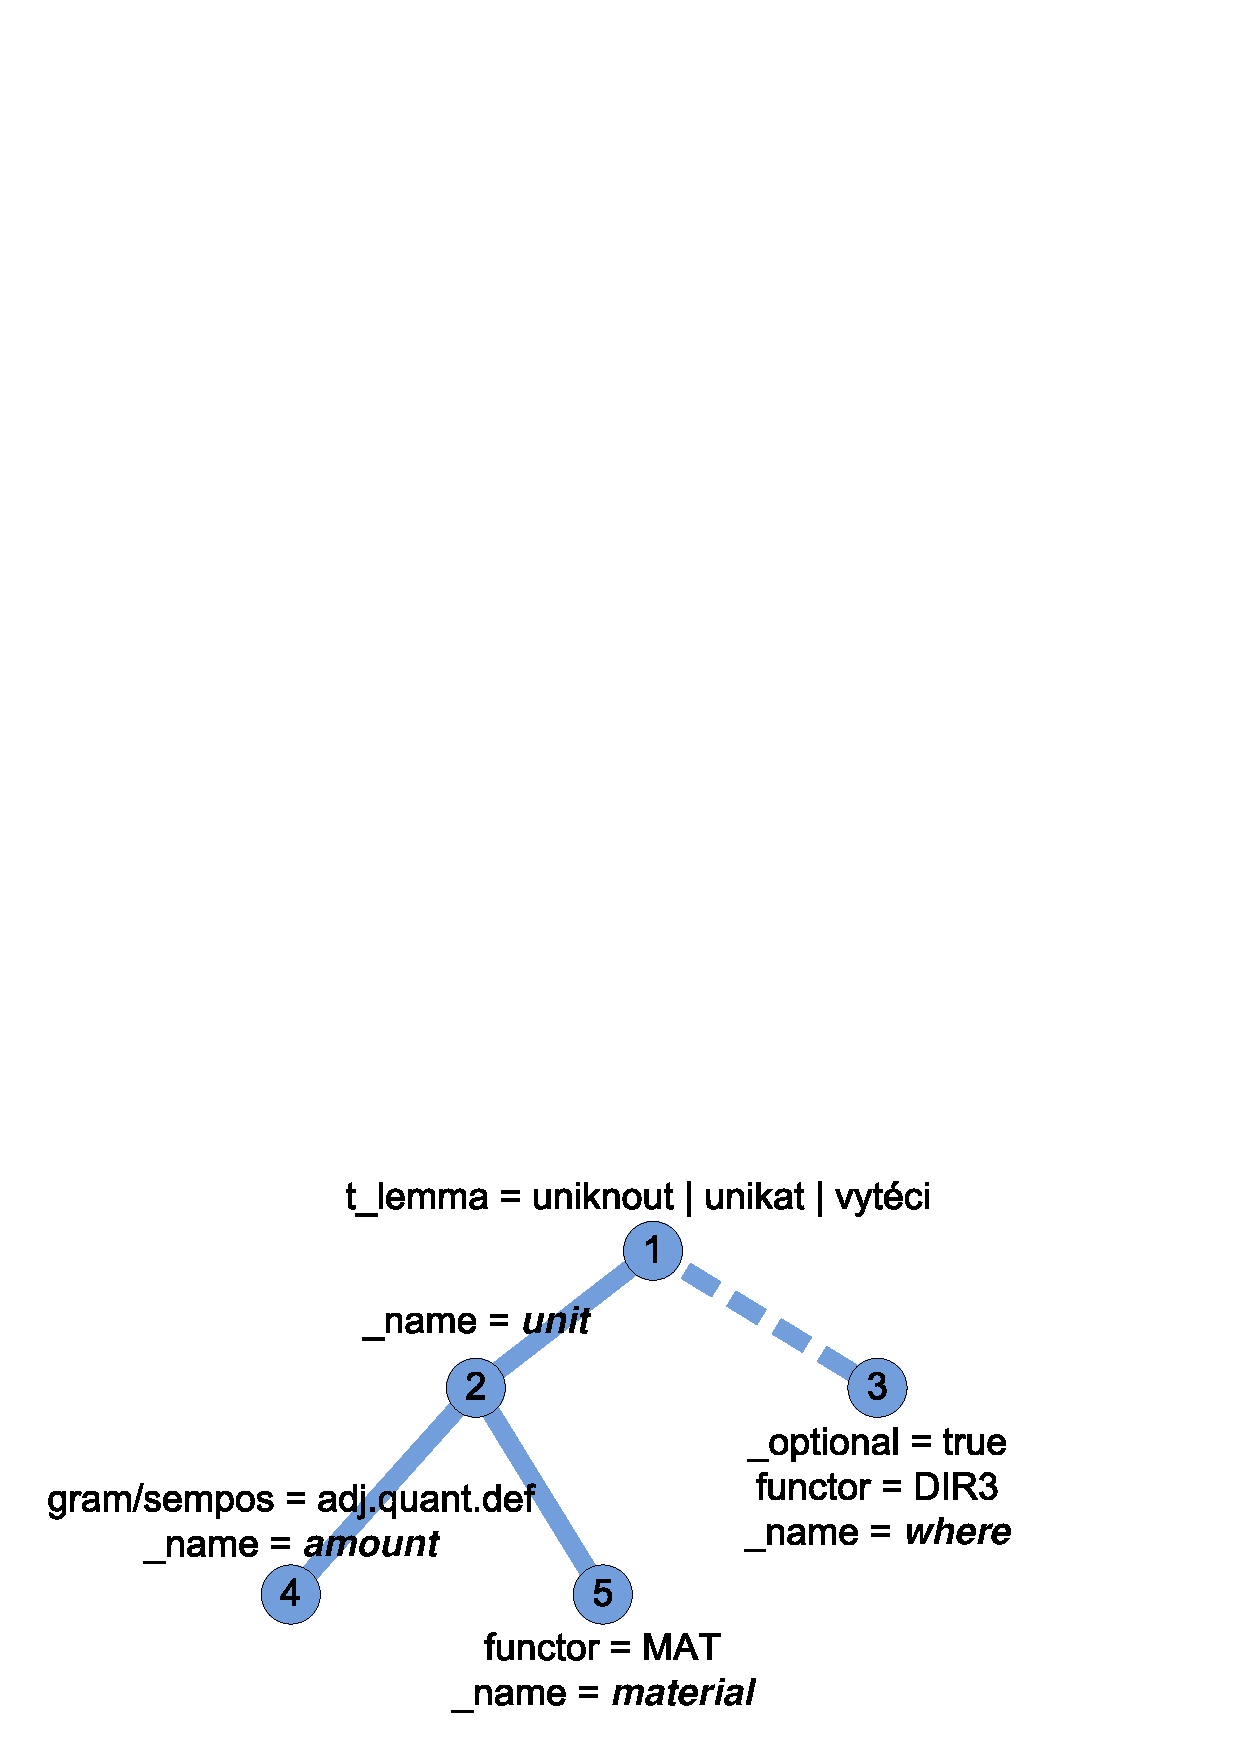
\includegraphics[height=0.6\vsize]{img/eenv_extr_rule}
\end{center}
%\begin{itemize}
%	\item Tree patterns on \alert{shape} and \alert{nodes} (on node attributes).
%	\item Evaluation gives \alert{actual matches} of particular nodes.
%	\item \alert{Names} of nodes allow use of references.
%\end{itemize}
\end{frame}



\begin{frame}{Matching Tree}
%\begin{center}
\centerline{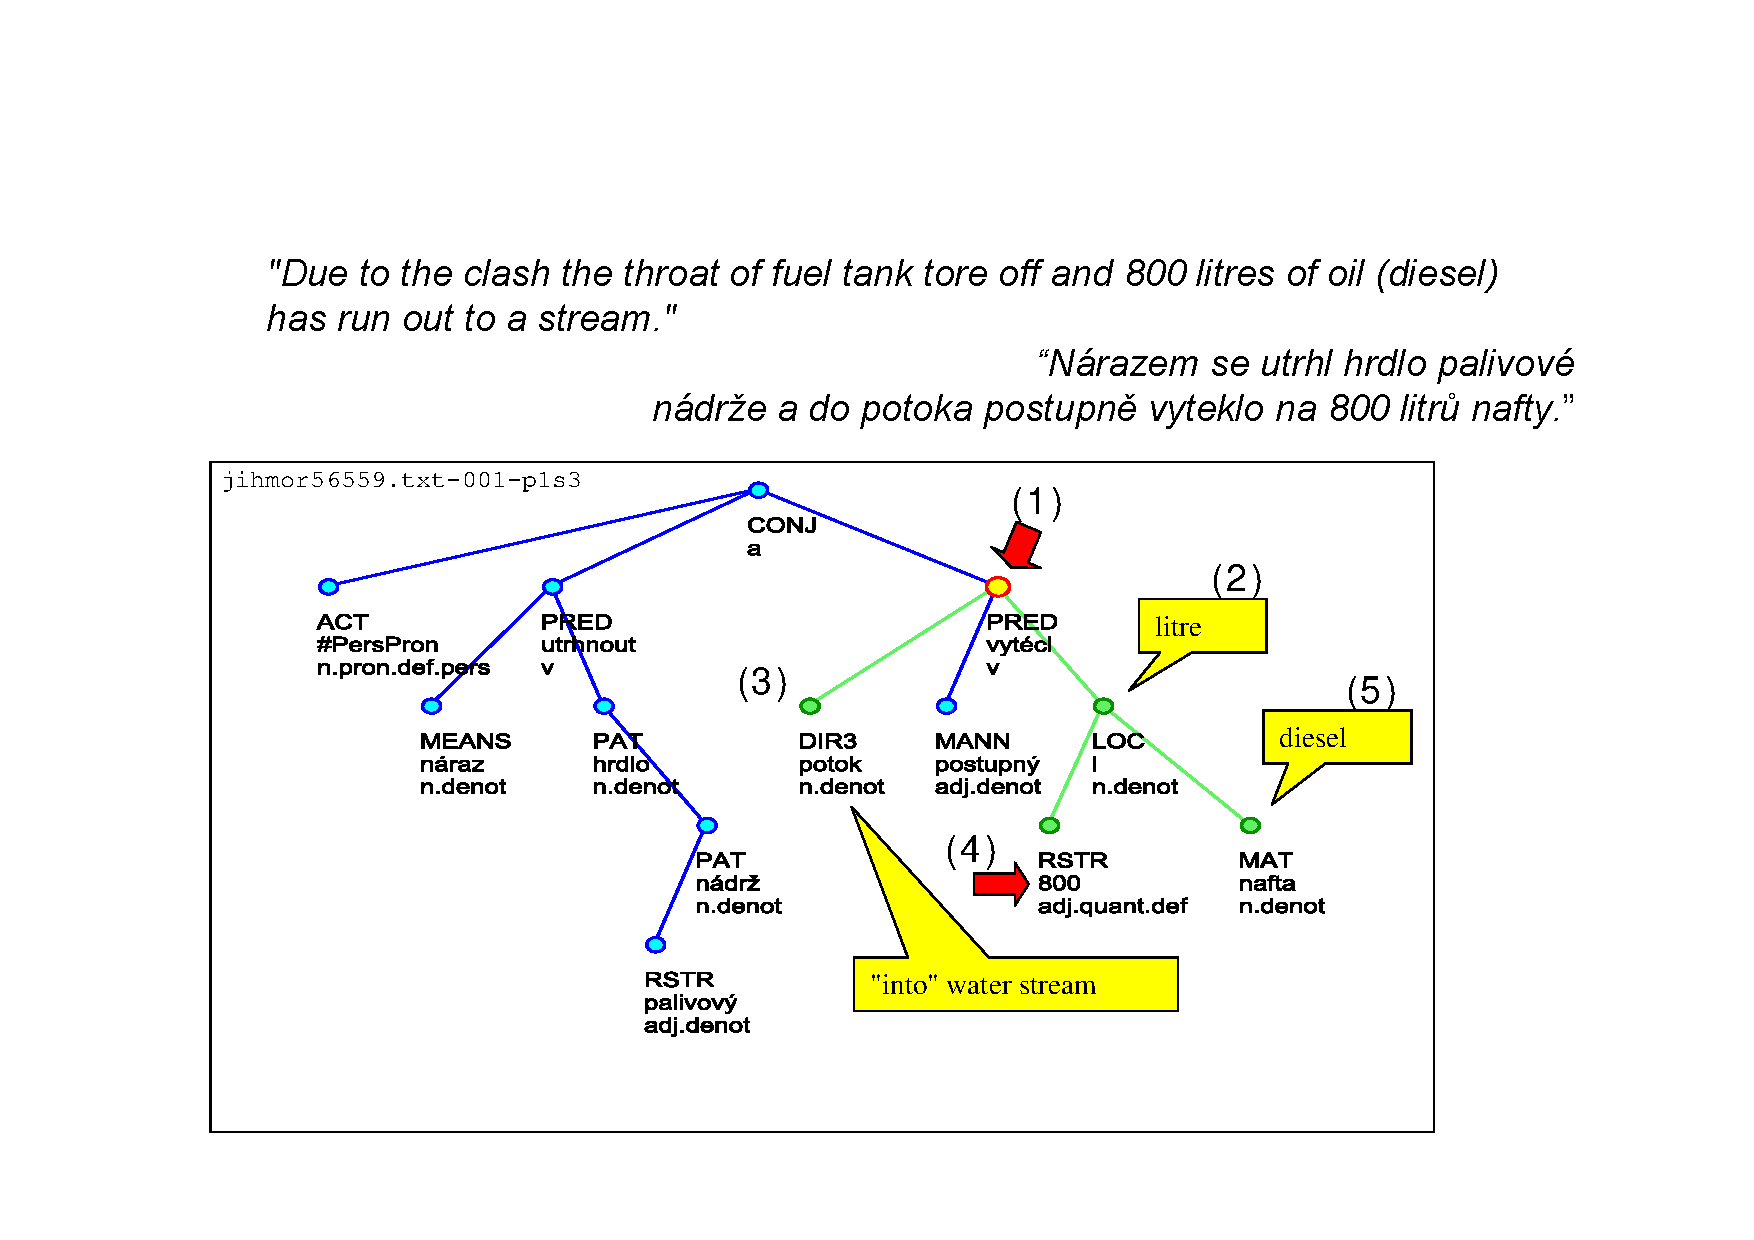
\includegraphics[height=0.8\vsize]{img/eenv_tree}}
%\end{center}
%{\scriptsize
%\textbf{SELECT} \alert{action\_type}.t\_lemma, \alert{a-negation}.m\/tag, 
%\alert{injury\_manner}.t\_lemma, \alert{participant}.t\_lemma,
%\alert{quantity}.t\_lemma \textbf{FROM} \emph{***extraction rule***} 
%}
\end{frame}


\begin{frame}{Raw data extraction output}
%\begin{center}
\centerline{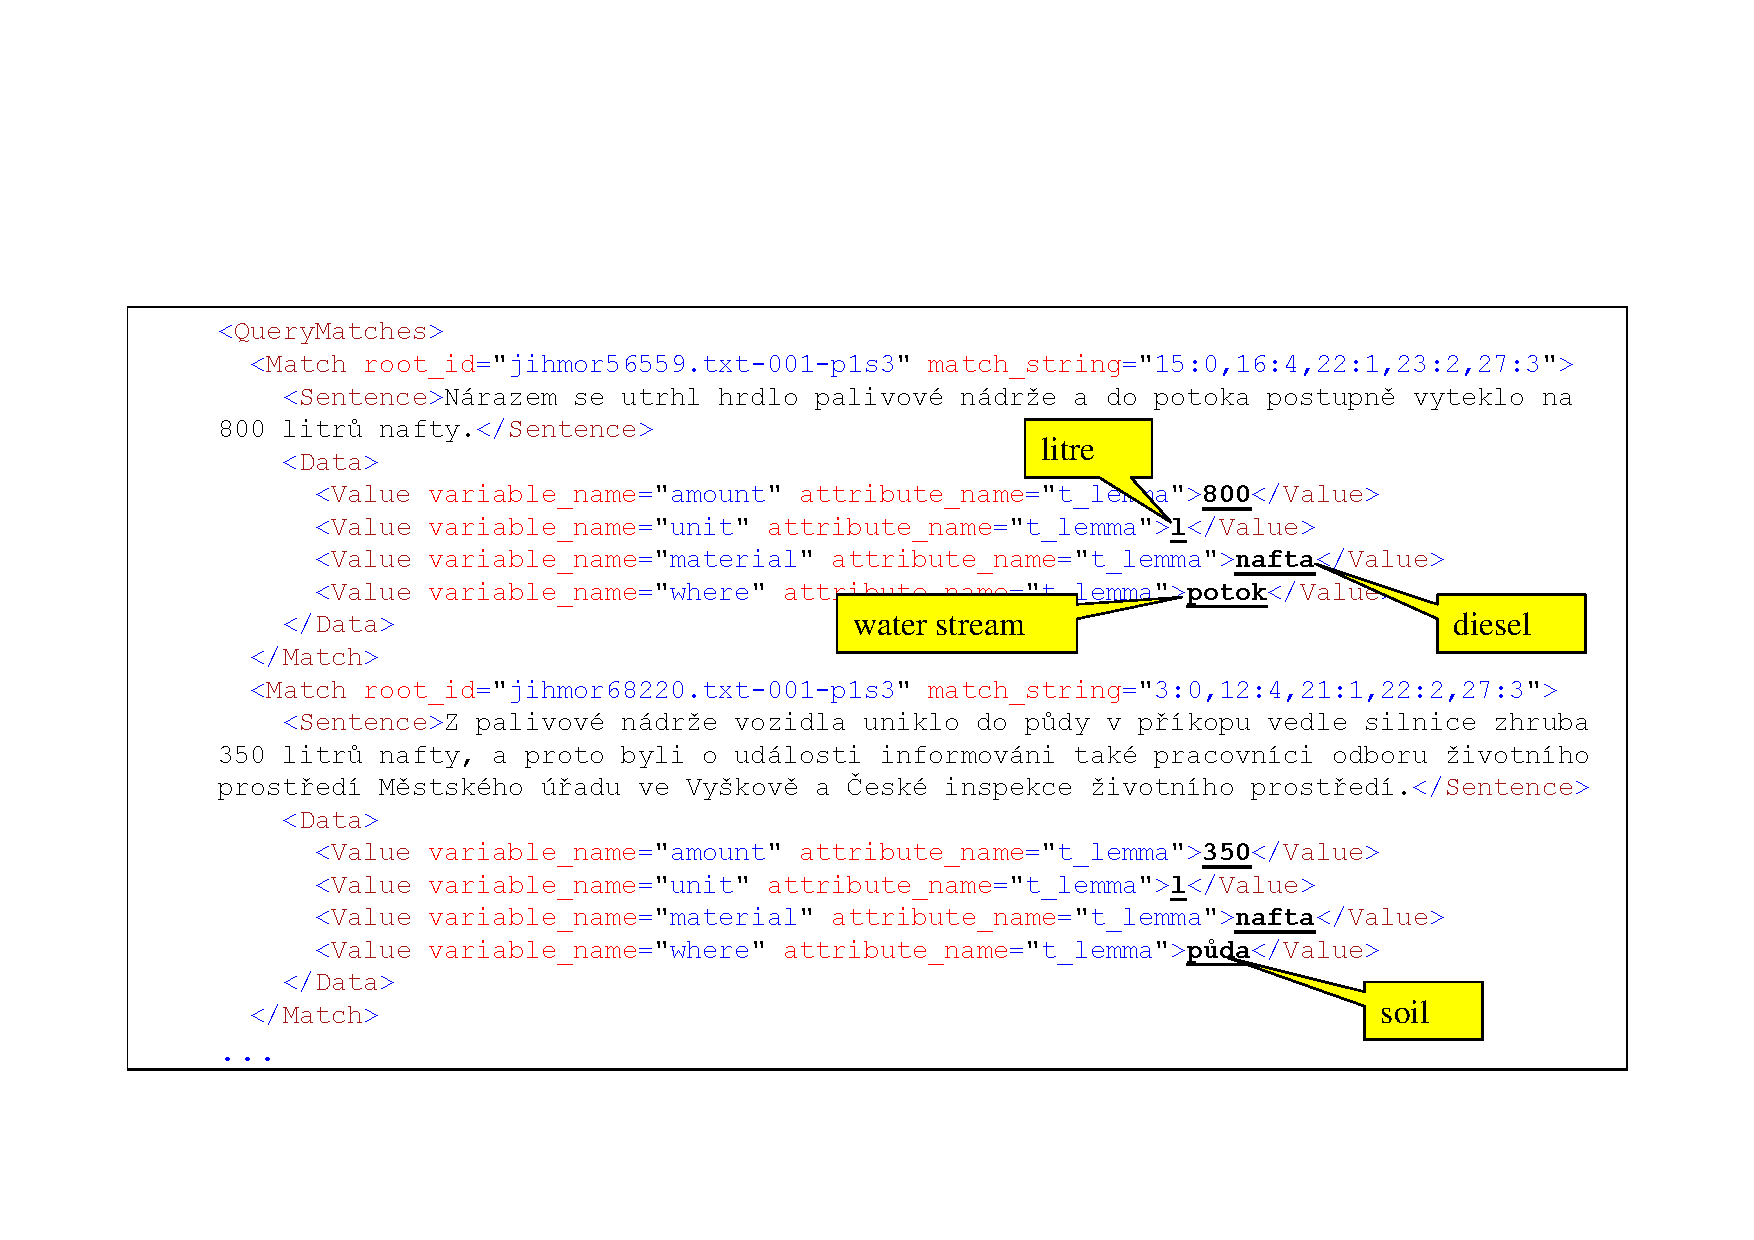
\includegraphics[height=0.77\vsize]{img/eenv_results}}
%\end{center}
{\scriptsize
\textbf{SELECT} \alert{amount}.t\_lemma, \alert{unit}.t\_lemma, 
\alert{material}.t\_lemma, \alert{where}.t\_lemma
\\ \textbf{FROM} \emph{***extraction rule***} 
}
\end{frame}



\begin{frame}{Design of extraction rules -- iterative process}
\begin{center}
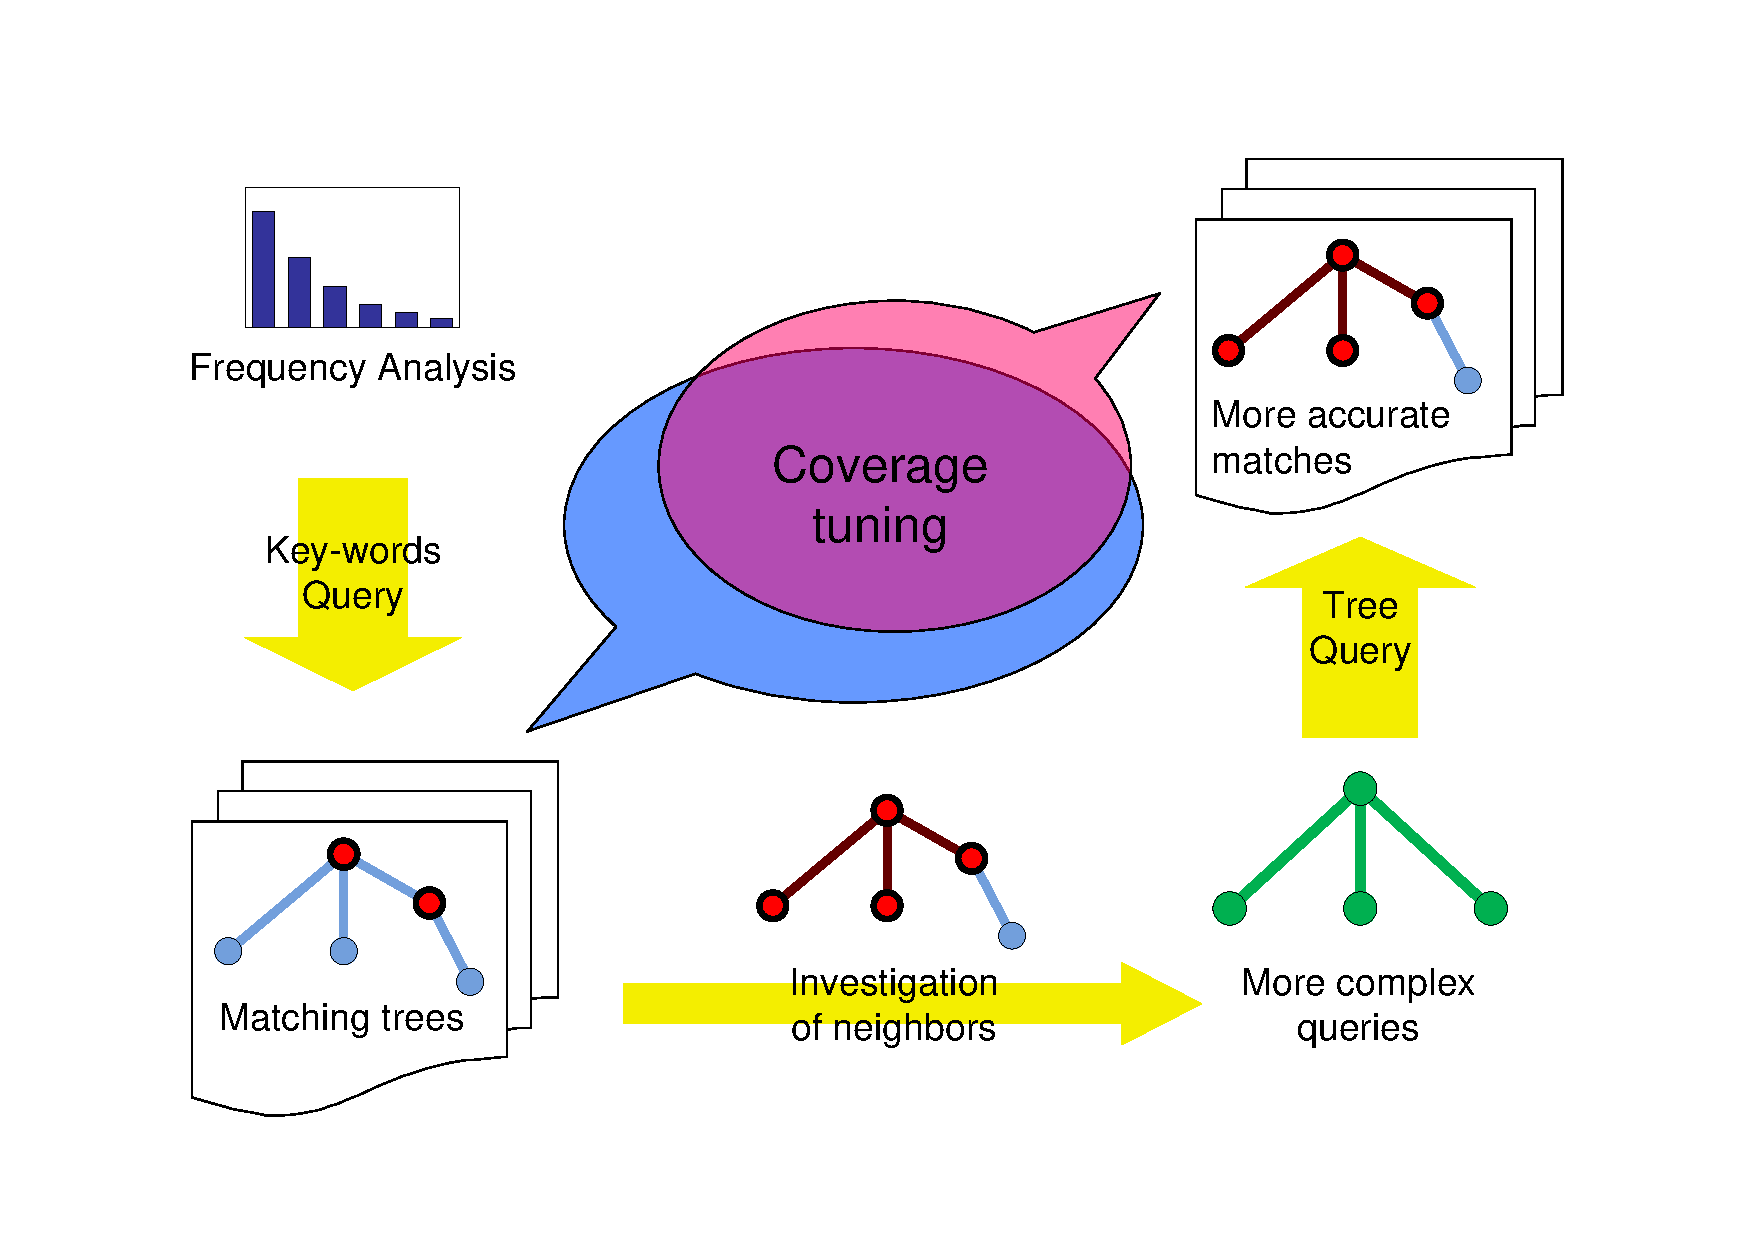
\includegraphics[height=0.6\vsize]{img/coverge_tuning}
\end{center}
\begin{enumerate}
	\item \alert{Frequency analysis} $\rightarrow$ representative key-words.
	\item Investigating of matching trees $\rightarrow$ \alert{tuning} of tree query.
	\item \alert{Complexity} of the query $\cong$ complexity of extracted data.
\end{enumerate}
\end{frame}



\subsection{Induction of Extraction Rules}
\themecolor{\colorLearning}
\frame{\frametitle{Induction of Extraction Rules} \tableofcontents[currentsubsection]}

\subsection{Shareable Extraction Ontologies}
\themecolor{\colorShareable}
\frame{\frametitle{Shareable Extraction Ontologies} \tableofcontents[currentsubsection]}

\subsection{Fuzzy ILP Document Classification}
\themecolor{\colorFuzzy}
\frame{\frametitle{Fuzzy ILP Document Classification} \tableofcontents[currentsubsection]}


\resetcolor
\section[Questions \& Comments]{Questions and Comments from Reviews} 
\frame{\tableofcontents[currentsection]}

\begin{frame}{The Task of Information Extraction}
\begin{itemize}
	\item Is it really necessary to discuss all these topics?	
	\begin{itemize}
		\item Are we presenting our work or creating a ``text book''?
	\end{itemize}	
	\item What reference is actually missing?
	\item Is the used terminology lacking something important?
\end{itemize}
\begin{center}
	\begin{tabular}{l|l}
		Dědek & MUC-6 1995, Appelt \& Israel 1999\\
		\hline
		\emph{Entity Recognition} & Named Entity Recognition\\
		Relation Extraction & Template Element Construction\\
		Event Extraction & Template Relation Construction	\\
		\textbf{Event Extr. Encoded as Ent. Rec.} & Template Unification\\
		Instance Resolution & Scenario Template Production
	\end{tabular}
\end{center}
\end{frame}



\begin{frame}{Available Resources Criterion:\\Time, Effort, Allocated Capabilities}
\begin{itemize}
	\item One common answer to comments like:	
	\begin{itemize}
		\item ``Chapter, section, etc. is too short.''
		\item ``Problem, solution, etc. should be more discussed.''
		\item ``The techniques could easily be described and motivated in much more detail.''
		\item ``More examples should be given.''
		\item ``Evaluation dataset is rather too small.''
	\end{itemize}
	

	\item The answer is:		
	\begin{itemize}
		\item Yes, that is reasonable comment, but there were no more available resources for it.
		\item Is the work as a whole too short?
		\item Are there parts that should have been omitted?
		\medskip
		\item We did our best to include the most important and relevant things.
		\item But then, oops, the time was up! 
	\end{itemize}

	\item Let's look at this in more detail on the next slide...		
\end{itemize}
\end{frame}

\begin{frame}{Available Resources and Allocated Capabilities}
\begin{itemize}
	\item Full time Ph.D. Student (4 years)
	\begin{itemize}
		\item In the beginning usually not yet skilled researcher in given topic
	\end{itemize}	
	\item Studying duties and activities
	\begin{itemize}
		\item There are so many interesting subjects not possible to attend because of lack of time 
	\end{itemize}	
	\item Teaching duties	
	\begin{itemize}
		\item Preparation of lecture materials
		\item Student's homeworks, exams
	\end{itemize}	
	\item Writing papers 
	\begin{itemize}
		\item Not always completely relevant to the Ph.D. topic
	\end{itemize}
	\item Presentations, conferences
	\begin{itemize}
		\item Preparations
		\item Traveling
	\end{itemize}
	\item Writing reviews 
	\begin{itemize}
		\item Student's thesis
		\item Research papers
	\end{itemize}
	\item Internship?
	\medskip
	\item Active research
	\begin{itemize}
		\item Optimistic balance: remaining 30\% of available resources (not only time)
		%\item Searching for existing approaches and studying them
		%\item Working with new technologies
		%\item Software development
	\end{itemize}
	
\end{itemize}
\end{frame}


\end{document}
